% ======================================================================
% DISEÑO E IMPLEMENTACIÓN
% ======================================================================
\section{Diseño e Implementación}
\label{ch:diseno-implementacion}

El capítulo anterior estableció los formalismos que fundamentan la extensión:
la Programación Lógica Probabilística, las Disyunciones Anotadas y el Conteo
de Modelos Ponderados. Este capítulo transforma esos conceptos en artefactos
de software. La Sección~\ref{sec:di-analisis-arquitectura} analiza la
arquitectura original; la Sección~\ref{sec:di-retrocompatibilidad} demuestra
la retrocompatibilidad con los modelos booleanos existentes. Las
Secciones~\ref{sec:di-fluentschema} a~\ref{sec:di-herramientas} describen el
esquema factorizado del espacio de estados, el clasificador automático de
fluentes, el \textit{pipeline} de preparación del MDP, la adaptación del
algoritmo de Iteración de Valor, el evaluador de Darwiche y los módulos de
soporte.

% ------------------------------------------------------------------
\subsection{Análisis de la arquitectura original}
\label{sec:di-analisis-arquitectura}

El punto de partida de cualquier extensión es comprender la arquitectura que se
extiende. MDP-ProbLog opera bajo un diseño modular que separa la inferencia
probabilística, la representación del espacio de estados, la orquestación del MDP
y la resolución numérica en módulos con responsabilidades delimitadas~\cite{bueno2016mdp}.
El análisis de esta arquitectura permite identificar dónde reside la
restricción booleana y qué módulos requiere modificar la extensión.

\subsubsection{Componentes del sistema original}
\label{sec:di-arquitectura-base}

% [FIGURA]: Diagrama de bloques de la arquitectura original.
%   Tipo: Diagrama de bloques.
%   Contenido: Cuatro rectángulos etiquetados engine.py, fluent.py, mdp.py,
%     value_iteration.py. Flechas de dependencia saliendo de mdp.py hacia los
%     otros tres módulos. engine.py contiene una caja interna con "ClauseDB"
%     y "Compilador ProbLog". fluent.py contiene "StateSpace (binario)".
%   Relación: Referenciado como "La Figura~\ref{fig:arquitectura-original}
%     muestra la arquitectura del sistema original."
%   Justificación: Cuatro módulos con dependencias unidireccionales son más
%     claros en un diagrama de bloques que en prosa.
%   Label sugerido: fig:arquitectura-original

La arquitectura original separa las responsabilidades del \textit{framework} en
cuatro módulos. Cada módulo tiene una función delimitada y las dependencias fluyen
en una sola dirección. La Figura~\ref{fig:arquitectura-original} exhibe
esta estructura; la responsabilidad de cada módulo se detalla a continuación.

\begin{description}
    \item[\texttt{engine.py}] Implementa un adaptador sobre el motor interno de
        ProbLog (\texttt{DefaultEngine}). Encapsula la Base de Datos de Cláusulas
        (\texttt{ClauseDB}) y expone métodos para añadir hechos lógicos, ejecutar
        el \textit{grounding} relevante y compilar circuitos evaluables para el
        Conteo de Modelos Ponderados.

    \item[\texttt{fluent.py}] Define las abstracciones del estado del sistema. Las
        clases \texttt{Fluent} y \texttt{StateSpace} generan e indexan las
        configuraciones posibles del espacio de estados, asumiendo un dominio
        factorizado puramente booleano.

    \item[\texttt{mdp.py}] Actúa como coordinador del \textit{framework}. Interroga
        la \texttt{ClauseDB} buscando predicados reservados
        (\texttt{state\_fluent/1}, \texttt{action/1}, \texttt{utility/2}), coordina
        la incorporación de hechos temporales y traduce las relaciones lógicas en
        una semántica de transiciones de Markov.

    \item[\texttt{value\_iteration.py}] Implementa el algoritmo de Iteración de
        Valor. Opera sobre índices enteros y distribuciones marginales para calcular
        la función de valor óptima mediante la ecuación de optimalidad de Bellman.
\end{description}

\begin{figure}[H]
    \centering
    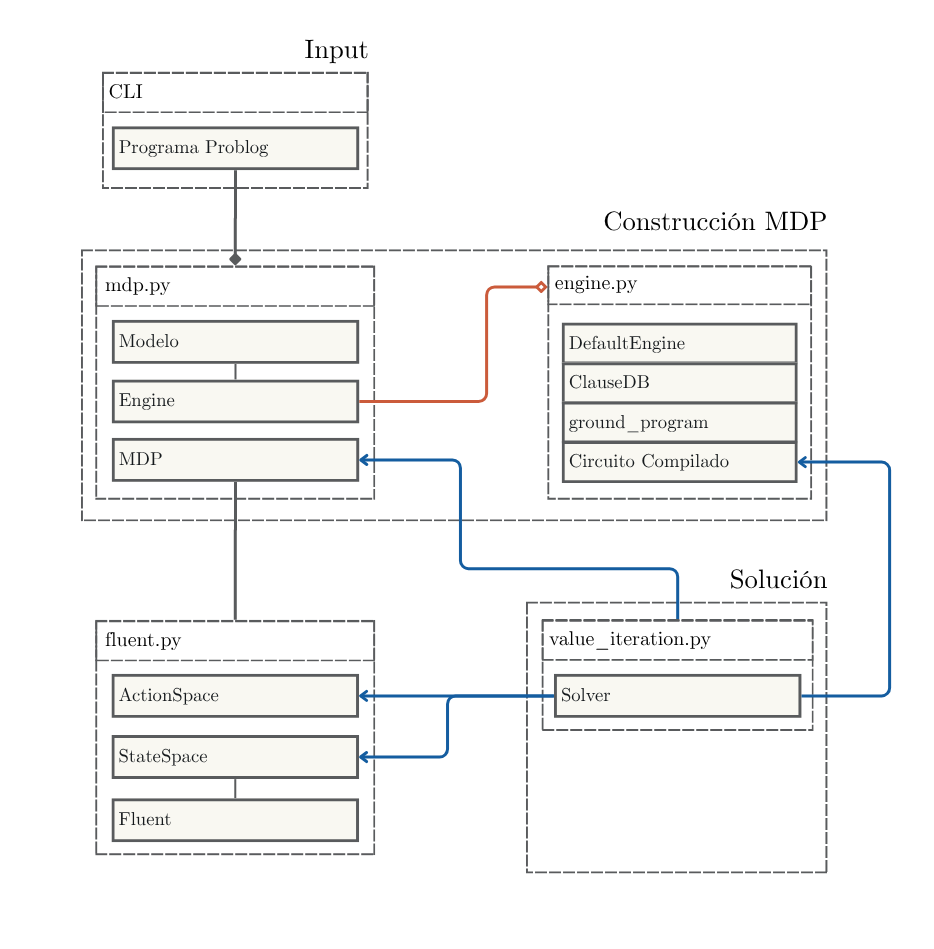
\includegraphics[width=0.80\textwidth]{figuras/arqui-original.png}
    \caption{Diagrama de la arquitectura original del framework MDP-ProbLog.}
    \label{fig:arquitectura-original}
\end{figure}


El módulo \texttt{mdp.py} depende de \texttt{engine.py}, \texttt{fluent.py}
y \texttt{value\_iteration.py}. Los módulos \texttt{engine.py} y
\texttt{fluent.py} son independientes entre sí. Esta organización delimita el
alcance de la extensión: \texttt{fluent.py} y \texttt{mdp.py} son los
candidatos a modificación; \texttt{engine.py} permanece inalterado.

\subsubsection{Flujo de ejecución}
\label{sec:di-flujo-ejecucion}

La interacción entre estos módulos sigue un flujo de cinco fases:

\begin{enumerate}
    \item \textbf{Análisis y carga.} El módulo \texttt{engine.py} realiza el
        \textit{parsing} del archivo Prolog proporcionado por el usuario y lo
        inyecta en la \texttt{ClauseDB}.

    \item \textbf{Descubrimiento del dominio.} El coordinador \texttt{mdp.py}
        interroga la \texttt{ClauseDB} para identificar los fluentes de estado y
        las acciones declaradas, e instancia los iteradores correspondientes en
        \texttt{fluent.py}.

    \item \textbf{Inyección temporal.} Para modelar la dinámica secuencial,
        \texttt{mdp.py} convierte las declaraciones abstractas en versiones con
        marca de tiempo ($t = 0$ para el estado actual, $t = 1$ para el siguiente
        estado). En esta fase se introducen hechos probabilísticos neutrales en
        $t = 0$ que serán reemplazados por evidencia determinista durante la
        evaluación de cada par estado-acción.

    \item \textbf{Aterrizado y compilación.} Se ejecuta un \textit{grounding}
        relevante respecto a las consultas de interés. Las reglas de transición se
        compilan en un circuito proposicional evaluable (SDD o d-DNNF, según el
        \textit{backend} seleccionado).

    \item \textbf{Resolución.} El módulo \texttt{value\_iteration.py} recorre el
        espacio de estados, inyecta cada par estado-acción como evidencia en el
        motor y solicita las probabilidades marginales $P(s' \mid s, a)$ mediante
        WMC para actualizar la función de valor $V(s)$.
\end{enumerate}

Dos de estas cinco fases asumen implícitamente un dominio booleano. La Fase~3
inyecta hechos probabilísticos independientes para cada fluente, presuponiendo
que cada variable de estado tiene dominio $\{0, 1\}$. La Fase~5 recorre un
espacio de estados construido como el producto cartesiano de factores binarios.
La extensión modifica estas dos fases y la estructura de datos que las sustenta.


\subsubsection{Limitaciones en la gestión de fluentes}
\label{sec:di-limitaciones-gestion}

Forzar fluentes categóricos en variables de Bernoulli degrada el modelado
lógico y la eficiencia computacional por la explosión de estados espurios,
como se estableció en el Capítulo~\ref{ch:marco-teorico}.

El diseño original implementa \texttt{StateSpace} como un iterador combinatorio
plano que procesa las declaraciones \texttt{state\_fluent/1} y genera
mecánicamente el producto cartesiano del dominio binario sin considerar el
agrupamiento ni la exclusión mutua.

La solución no requiere alterar el motor de inferencia de ProbLog. La
compilación a circuitos y el WMC permanecen intactos. La intervención ocurre
en la capa intermedia donde las declaraciones lógicas se transforman en
variables de estado evaluables para el \textit{solver}.

Se identifican tres puntos de extensión para integrar el soporte de fluentes
multivaluados:

\begin{enumerate}
    \item \textbf{Representación del espacio de estados.} Reemplazar \texttt{StateSpace}
        por una estructura factorizada que admita factores de cardinalidad arbitraria,
        eliminando la generación de combinaciones inválidas.

    \item \textbf{Inyección de hechos en la \texttt{ClauseDB}.} Adaptar la Fase~3
        del \textit{pipeline} para que los fluentes multivaluados se representen como
        Disyunciones Anotadas en lugar de hechos probabilísticos independientes.

    \item \textbf{Cálculo del valor esperado.} Reestructurar la evaluación del valor
        futuro en la Iteración de Valor para que recorra los factores del esquema en
        lugar de enumerar combinaciones binarias.
\end{enumerate}

% ------------------------------------------------------------------
\subsection{Esquema factorizado del espacio de estados}
\label{sec:di-fluentschema}

El primer componente a diseñar es la estructura de datos que reemplaza a
\texttt{StateSpace}. La clase \texttt{FluentSchema} admite factores de
cardinalidad arbitraria y expone operaciones uniformes de indexación y
decodificación accesibles desde cualquier módulo del \textit{framework}.

\subsubsection{Modelo de datos}
\label{sec:di-fluentschema-modelo}

El \texttt{FluentSchema} organiza el espacio de estados como una secuencia ordenada
de $m$ factores independientes. Cada factor $k$ es una lista de términos lógicos
aterrizados que representan las opciones mutuamente excluyentes de esa variable de
estado. La cardinalidad del factor $k$, denominada base $b_k$, es igual al número
de opciones que contiene.

La clase mantiene tres estructuras internas:

\begin{enumerate}
    \item \textbf{Lista de factores.} Una lista de listas de términos: el factor $k$
        contiene los $b_k$ términos que representan sus opciones. La posición de
        cada término dentro de su factor determina su índice local
        $v_k \in [0, b_k - 1]$.

    \item \textbf{Lista de bases.} Un arreglo de enteros $[b_1, b_2, \ldots, b_m]$
        que registra la cardinalidad de cada factor. Los factores booleanos tienen
        base~2; los factores multivaluados tienen base $N \geq 2$.

    \item \textbf{Lista aplanada.} La concatenación de todos los términos en orden
        de registro. Esta lista localiza cualquier término desde su índice global
        sin recorrer todos los factores.
\end{enumerate}

Dos categorías de factor se distinguen semánticamente. Un \textbf{factor booleano}
tiene base~2 y sus dos términos corresponden a los valores $\{0, 1\}$ de un fluente
de Bernoulli. Un \textbf{factor multivaluado} tiene base $N \geq 2$ y sus $N$
términos codifican los valores de una variable categórica en formato
\textit{one-hot}. Esta distinción determina la forma de inyección de hechos en
el \textit{pipeline} de preparación. Los factores booleanos se inyectan como
hechos probabilísticos independientes; los multivaluados, como Disyunciones
Anotadas.

\subsubsection{Codificación \textit{mixed-radix}}
\label{sec:di-mixed-radix}

El \texttt{FluentSchema} asigna a cada configuración un índice entero
$I \in [0, |\mathcal{S}| - 1]$ con codificación de base mixta
(\textit{mixed-radix}). Esta codificación generaliza la codificación binaria;
en lugar de base~2 uniforme, cada factor $k$ usa su propia base $b_k$.

El tamaño total del espacio de estados es el producto de todas las bases:
\begin{equation}
    |\mathcal{S}| = \prod_{k=1}^{m} b_k
    \label{eq:tamano-espacio}
\end{equation}

Para mapear una configuración a un índice, se calcula un \textit{stride} $S_k$ por
factor, definido como el producto de las bases de todos los factores que lo preceden:
\begin{equation}
    S_k = \prod_{i=1}^{k-1} b_i \quad \text{con } S_1 = 1
    \label{eq:strides}
\end{equation}

Dada una configuración donde el factor $k$ toma el valor local $v_k \in [0, b_k - 1]$,
el índice global se obtiene como:
\begin{equation}
    I = \sum_{k=1}^{m} v_k \times S_k
    \label{eq:codificacion}
\end{equation}

La decodificación extrae el valor local $v_k$ de cada factor como el residuo de
$I$ módulo $b_k$:
\begin{equation}
    v_k = I \bmod b_k, \quad I \leftarrow \left\lfloor \frac{I}{b_k} \right\rfloor
    \label{eq:decodificacion}
\end{equation}

Ambas operaciones recorren los $m$ factores en tiempo $O(m)$. La codificación
garantiza que cada índice $I \in [0, |\mathcal{S}| - 1]$ corresponde a exactamente
una combinación semánticamente válida. Los estados espurios son imposibles: la codificación no genera índices para
combinaciones inválidas.

\subsubsection{Ejemplo mixed-radix}
\label{sec:di-mixed-radix-ejemplo}

El ejemplo siguiente usa un dominio con dos variables de estado: \textbf{color},
con valores $\{\texttt{rojo}, \texttt{verde}, \texttt{azul}\}$, y
\textbf{velocidad}, con valores $\{\texttt{lenta}, \texttt{rápida}\}$. El
\texttt{FluentSchema} registra un factor de base~3 para color y uno de base~2
para velocidad.

El tamaño del espacio es $|\mathcal{S}| = 3 \times 2 = 6$, frente a los $2^5 = 32$
estados que generaría la codificación booleana equivalente con cinco fluentes
independientes. Los \textit{strides} son $S_1 = 1$ y $S_2 = 3$. La
Tabla~\ref{tab:mixed-radix-ejemplo} lista los seis estados resultantes.

\begin{table}[ht]
\centering
\caption{Codificación \textit{mixed-radix} para el dominio color $\times$ velocidad.}
\label{tab:mixed-radix-ejemplo}
\begin{tabular}{cccc}
\hline
\textbf{Índice $I$} & \textbf{color ($v_1$)} & \textbf{velocidad ($v_2$)} & \textbf{Cálculo} \\
\hline
0 & \texttt{rojo}\ (0)  & \texttt{lenta}\ (0)  & $0{\times}1 + 0{\times}3 = 0$ \\
1 & \texttt{verde}\ (1) & \texttt{lenta}\ (0)  & $1{\times}1 + 0{\times}3 = 1$ \\
2 & \texttt{azul}\ (2)  & \texttt{lenta}\ (0)  & $2{\times}1 + 0{\times}3 = 2$ \\
3 & \texttt{rojo}\ (0)  & \texttt{rápida}\ (1) & $0{\times}1 + 1{\times}3 = 3$ \\
4 & \texttt{verde}\ (1) & \texttt{rápida}\ (1) & $1{\times}1 + 1{\times}3 = 4$ \\
5 & \texttt{azul}\ (2)  & \texttt{rápida}\ (1) & $2{\times}1 + 1{\times}3 = 5$ \\
\hline
\end{tabular}
\end{table}

Por ejemplo, el estado con \texttt{azul} y \texttt{rápida} se codifica como
$I = 2 \times 1 + 1 \times 3 = 5$. La decodificación parte de $I = 5$: el color
se extrae como $5 \bmod 3 = 2$ (\texttt{azul}) y se actualiza $I \leftarrow
\lfloor 5 / 3 \rfloor = 1$; la velocidad se extrae como $1 \bmod 2 = 1$
(\texttt{rápida}). La decodificación concluye al agotar los factores.

\subsubsection{Operaciones relevantes}
\label{sec:di-fluentschema-ops}

Dos operaciones del \texttt{FluentSchema} son invocadas recurrentemente por el
resto del \textit{framework}:

\begin{description}
    \item[\texttt{get\_factors\_at(timestep)}] Retorna la lista de factores con los
        términos marcados con la estampa de tiempo indicada. \texttt{mdp.py} la
        invoca para obtener los factores del estado actual ($t = 0$) y del
        siguiente ($t = 1$) durante la preparación del \textit{pipeline}.

        El marcado temporal agrega el argumento entero $t$ como último argumento
        de cada término; el término \texttt{color(rojo)} a tiempo $t = 1$ se
        convierte en \texttt{color(rojo, 1)}.

    \item[\texttt{get\_local\_index(k, term)}] Dado el índice de factor $k$ y un
        término lógico aterrizado, retorna su posición $v_k$ dentro de ese factor.
        La Sección~\ref{sec:di-value-iteration} la invoca durante el recorrido
        recursivo de los factores. En cada nivel, traduce el término retornado
        por el evaluador a su posición $v_k$ para acumular el índice global del
        estado sucesor.
\end{description}

El \texttt{FluentSchema} centraliza la gestión del espacio de estados; los demás
módulos acceden a él exclusivamente por estas dos operaciones. El
\texttt{FluentClassifier} (Sección~\ref{sec:di-fluentclassifier}) lee las
declaraciones del programa lógico y construye el esquema de forma automática.


% ------------------------------------------------------------------
\subsection{Clasificador automático de fluentes}
\label{sec:di-fluentclassifier}

El \texttt{FluentSchema} debe construirse antes de que el \textit{framework}
ejecute cualquier otra etapa. Su construcción requiere conocer, para cada fluente
declarado, si pertenece a un factor booleano o a uno multivaluado. El predicado
\texttt{state\_fluent/1} declara la existencia del fluente, pero no su tipo. El
módulo \texttt{FluentClassifier} obtiene esa información de los nodos
\texttt{choice} que las Disyunciones Anotadas del programa dejan registrados en
la \texttt{ClauseDB}. El clasificador examina esos nodos, infiere el tipo de cada
fluente y construye el esquema sin intervención del usuario.

\subsubsection{Modos de declaración}
\label{sec:di-modos-declaracion}

El clasificador admite dos formas de declarar fluentes de estado. En el
\textbf{modo implícito}, el usuario escribe \texttt{state\_fluent(f(X))} y el
\textit{framework} infiere el tipo desde la estructura de la \texttt{ClauseDB}.
En el \textbf{modo explícito}, el usuario escribe
\texttt{state\_fluent(f(X),~multivalued)} o \texttt{state\_fluent(f(X),~bool)}
e indica el tipo directamente. El modo explícito tiene prioridad. Si un fluente
aparece en ambas formas, el \textit{framework} emite una advertencia y conserva
la declaración explícita.

El modo implícito es suficiente para la mayoría de los dominios. El modo
explícito es necesario en dominios con familias de variables indexadas por
entidad, como se discute al final de esta sección.

\subsubsection{El índice invertido de Disyunciones Anotadas}
\label{sec:di-indice-invertido}

La inferencia implícita depende de una estructura auxiliar denominada
\textbf{índice invertido}. El clasificador recorre la tabla de nodos de la
\texttt{ClauseDB} e identifica los nodos de tipo \texttt{choice}: las ramas
estocásticas que ProbLog genera para cada Disyunción Anotada. Por cada nodo
\texttt{choice}, extrae el término asociado y registra cada argumento constante
como clave del índice, bajo el identificador del grupo AD al que pertenece ese
nodo.

El resultado es un diccionario de la forma:
\begin{equation*}
    \mathcal{I} : \Sigma \to \mathcal{P}(\Gamma)
\end{equation*}
donde $\Sigma$ es el conjunto de valores constantes y $\Gamma$ es el conjunto de
identificadores de grupos AD. $\mathcal{I}(v)$ reúne los identificadores de los grupos AD que produjeron el
valor $v$.

La regla de transición siguiente ilustra la construcción del índice:

\begin{lstlisting}[language=Prolog]
0.7::color(rojo,1); 0.2::color(verde,1); 0.1::color(azul,1)
    :- color(rojo,0), cambiar.
\end{lstlisting}

ProbLog procesa esta AD y registra tres nodos \texttt{choice} bajo el grupo
$g_1$: uno para \texttt{color(rojo,1)}, uno para \texttt{color(verde,1)} y uno
para \texttt{color(azul,1)}. El clasificador extrae los argumentos constantes
de cada término y construye:
\[
    \mathcal{I}(\texttt{rojo}) = \{g_1\}, \quad
    \mathcal{I}(\texttt{verde}) = \{g_1\}, \quad
    \mathcal{I}(\texttt{azul}) = \{g_1\}
\]
Este índice queda disponible antes de que comience la clasificación.

\subsubsection{Pipeline de clasificación}
\label{sec:di-pipeline-clasificacion}

El método \texttt{classify()} ejecuta seis pasos secuenciales para construir el
\texttt{FluentSchema}:

\begin{enumerate}
    \item \textbf{Validación de declaraciones explícitas.} Se verifica que cada tag
        de tipo en las declaraciones \texttt{state\_fluent/2} sea \texttt{bool} o
        \texttt{multivalued}. Los tags inválidos se acumulan y se lanzan como un
        único error compuesto (\texttt{FluentDeclarationError}) para que el usuario
        pueda corregirlos todos de una vez.

    \item \textbf{Registro de fluentes explícitos.} Cada par
        \texttt{(término, tag)} se almacena en el registro explícito con su tipo
        ya conocido. Estos fluentes quedan excluidos de la inferencia implícita.

    \item \textbf{Registro de fluentes implícitos.} Los fluentes declarados con
        \texttt{state\_fluent/1} se agrupan por \texttt{(functor, aridad)}. Para
        cada grupo, se invoca \texttt{\_infer\_fluent\_type()}
        (Sección~\ref{sec:di-inferencia-tipo}) para determinar si el fluente es
        booleano o multivaluado.

    \item \textbf{Fusión de registros.} Los resultados de los pasos~2 y~3 se
        fusionan en un registro unificado. Las declaraciones explícitas
        sobrescriben las implícitas cuando coinciden en la misma clave.

    \item \textbf{Separación por tipo.} El registro se recorre en orden alfabético.
        Los fluentes booleanos se añaden al esquema con
        \texttt{schema.add\_bool(term)}. Los fluentes multivaluados se acumulan por
        \textit{functor} en un buffer temporal.

    \item \textbf{Validación de cardinalidad.} Cada grupo multivaluado acumulado
        en el paso~5 se verifica: si contiene menos de dos opciones, se lanza un
        \texttt{FluentCardinalityError}, pues un factor de exclusión mutua requiere
        al menos dos alternativas. Los grupos válidos se registran con
        \texttt{schema.add\_group(terms)}.
\end{enumerate}

%   Diagrama de flujo del pipeline de clasificación de 6 pasos.
%   Tipo: Diagrama de flujo vertical con 6 cajas numeradas.
%   Contenido: Nombres de los pasos, flechas secuenciales, indicar qué
%     estructuras produce cada paso (explicit_registry, implicit_registry,
%     full_registry, FluentSchema parcial, FluentSchema validado).
%   Label sugerido: fig:pipeline-clasificacion

\begin{figure}[htbp]
    \centering
    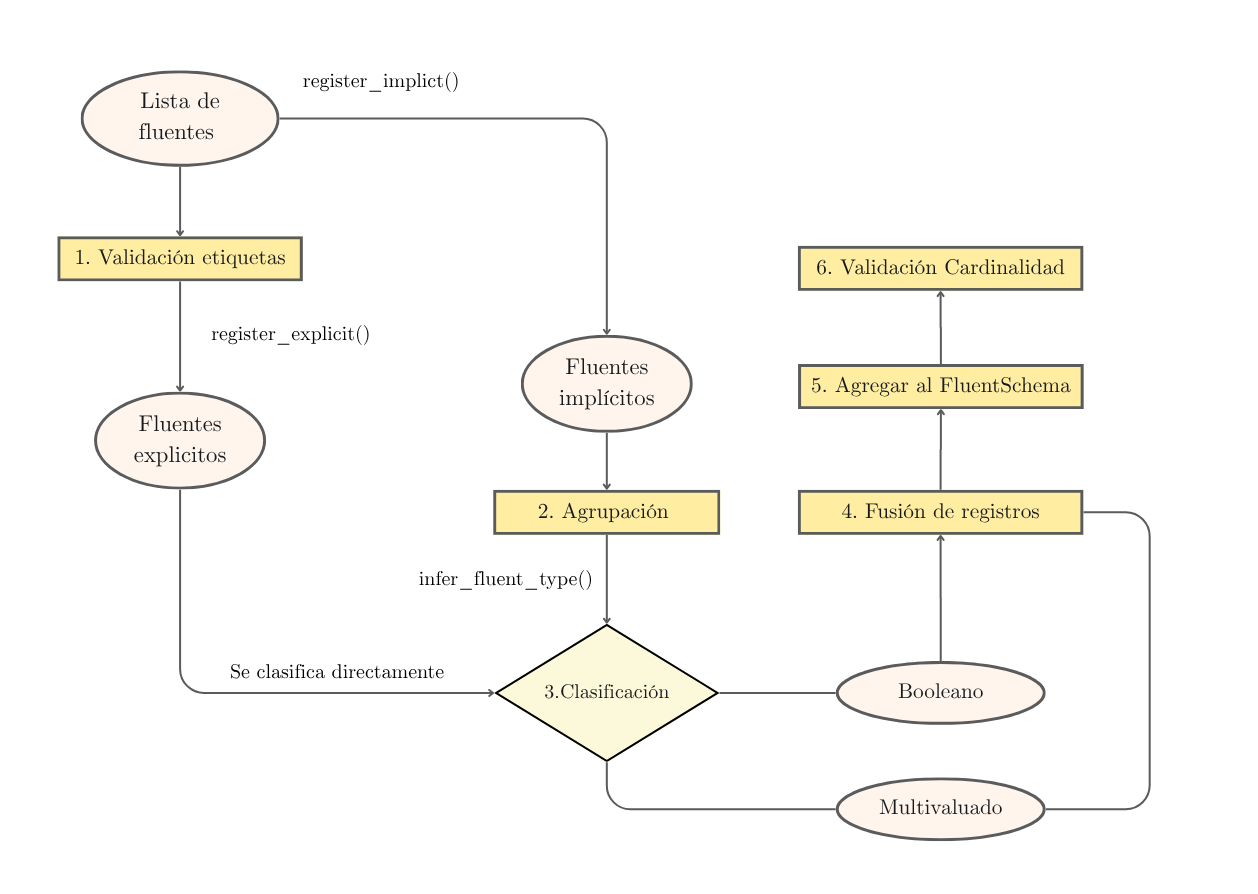
\includegraphics[width=1.0\textwidth]{figuras/pipeline-clasificacion.png} 
    \caption{pipeline de clasificación. Se explica la ejecución del método \texttt{classify()}}
    \label{fig:pipeline-clasificacion}
\end{figure}


\subsubsection{Inferencia implícita de tipo}
\label{sec:di-inferencia-tipo}

El paso~3 del \textit{pipeline} delega la decisión de tipo en
\texttt{\_infer\_fluent\_type()}. La función clasifica como booleano cualquier
fluente de aridad~0. Los fluentes proposicionales carecen de argumentos y son
binarios por definición. Si el fluente tiene aridad~$\geq 1$, la función examina
cada posición argumental $p$ del término. Para cada posición, extrae el conjunto
$V_p$ de valores que ese argumento toma en los términos aterrizados e intersecta
los grupos AD de cada valor. Una intersección no vacía indica que todos los valores
de la posición $p$ provienen de un mismo grupo AD; el fluente es multivaluado. Si
ninguna posición pasa esta prueba, el fluente es booleano.

El Algoritmo~\ref{alg:infer-type} formaliza esta lógica.

\begin{algorithm}[H]
\caption{Inferencia de tipo por intersección de orígenes estocásticos}
\label{alg:infer-type}
\begin{algorithmic}[1]
\Require Conjunto de términos aterrizados $G$ de aridad $a$; índice invertido
    $\mathcal{I}: \Sigma \to \mathcal{P}(\Gamma)$.
\Ensure Clasificación: \texttt{bool} o \texttt{multivalued}.

\If{$a = 0$}
    \Return \texttt{bool}
\EndIf

\For{$p \gets 1$ \textbf{a} $a$}
    \State $V_p \gets \{ \text{arg}_p(g) \mid g \in G \}$
    \State $C \gets \bigcap_{v \in V_p} \mathcal{I}(v)$
    \If{$C \neq \emptyset$}
        \Return \texttt{multivalued}
    \EndIf
\EndFor

\Return \texttt{bool}
\end{algorithmic}
\end{algorithm}

Aplíquese el algoritmo al fluente \texttt{color} del ejemplo anterior. Los términos aterrizados son \texttt{color(rojo)},
\texttt{color(verde)} y \texttt{color(azul)}, todos de aridad~1. En la
posición~0, los valores son $V_0 = \{\texttt{rojo}, \texttt{verde},
\texttt{azul}\}$. La intersección es:
\[
    \mathcal{I}(\texttt{rojo}) \cap \mathcal{I}(\texttt{verde}) \cap
    \mathcal{I}(\texttt{azul}) = \{g_1\} \neq \emptyset
\]
El algoritmo retorna \texttt{multivalued}. El fluente se registra como un factor de
base~3 en el esquema.

El agrupamiento del paso~5 es correcto para variables categóricas globales. En
esos dominios, todos los términos con el mismo \textit{functor} corresponden a
opciones de una única variable de estado. Cuando múltiples entidades comparten
predicado pero requieren independencia estocástica, el agrupamiento puede fusionar
factores que deberían ser independientes. En esos casos, la declaración explícita
con \texttt{state\_fluent/2} define cada factor por separado y evita la
consolidación automática.

Con el \texttt{FluentSchema} construido y validado, el \textit{framework} dispone
del espacio de estados necesario para el \textit{pipeline} de preparación del MDP
(Sección~\ref{sec:di-pipeline-mdp}).


% ------------------------------------------------------------------
\subsection{Pipeline de preparación del MDP}
\label{sec:di-pipeline-mdp}

El \textit{pipeline} de preparación transforma el \texttt{FluentSchema} en una
base de cláusulas evaluable bajo condicionamiento. Esta transformación ocurre en
el método \texttt{\_\_prepare()} de la clase \texttt{MDP}, antes de que comience
la Iteración de Valor.

\subsubsection{Fases del pipeline}
\label{sec:di-fases-pipeline}

\begin{enumerate}
    \item \textbf{Clasificación.} Se instancia el \texttt{FluentClassifier} para
        construir el \texttt{FluentSchema}. El resultado queda disponible para
        las fases siguientes.

    \item \textbf{Inyección de hechos \textit{dummy}.} Los hechos probabilísticos
        del estado actual ($t = 0$) se insertan en la \texttt{ClauseDB}, uno por
        factor del esquema. Estos hechos son \textit{dummy}: sus probabilidades
        son valores neutrales que serán sustituidos en cada evaluación
        individual.

    \item \textbf{Inyección de acciones.} Las acciones del modelo se inyectan
        como una Disyunción Anotada con distribución uniforme; la exclusión
        mutua queda garantizada por construcción.

    \item \textbf{Aterrizado relevante.} Se ejecuta un \textit{grounding}
        limitado a las consultas de interés: fluentes del siguiente estado
        ($t = 1$), utilidades, acciones y fluentes del estado actual ($t = 0$).
        Incluir los fluentes en $t = 0$ entre las consultas preserva sus
        identificadores en el circuito compilado; sin ellos, la sustitución de
        evidencia no podría localizar los nodos correctos.

    \item \textbf{Compilación del circuito.} Los fluentes del siguiente estado y
        las utilidades se compilan en un único circuito d-DNNF o SDD. El
        circuito queda fijo y se reutiliza en todas las evaluaciones.
\end{enumerate}

% [FIGURA]: Diagrama de flujo de las 5 fases del pipeline de preparación.
%   Tipo: Diagrama de flujo vertical con 5 cajas numeradas.
%   Contenido: Fases 1-5 con sus nombres. Flechas descendentes. Anotar qué
%     estructura produce cada fase: FluentSchema, ClauseDB con dummy, circuito.
%   Label sugerido: fig:pipeline-preparacion

\begin{figure}[H]
    \centering
    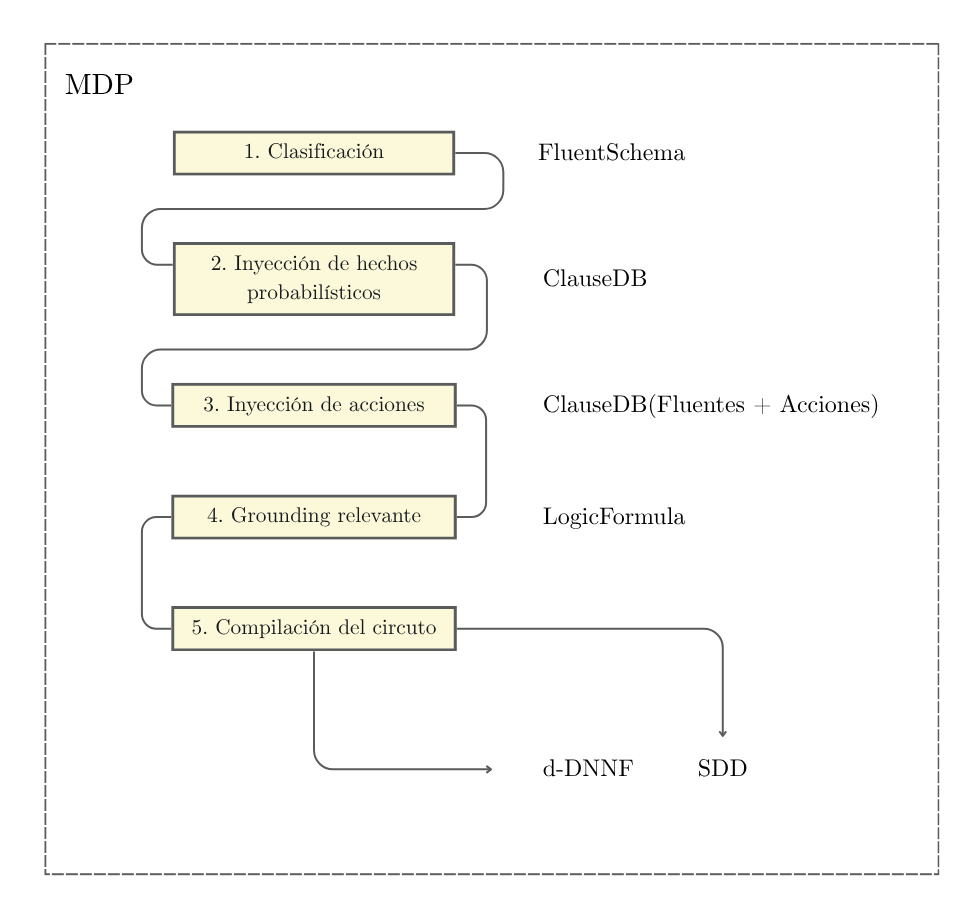
\includegraphics[width=0.80\textwidth]{figuras/pipeline-preparacion.png} 
    \caption{pipeline de preparación. Se explica la ejecución del método \texttt{\_\_prepare()}}
    \label{fig:pipeline-preparación}
\end{figure}

\subsubsection{Hechos \textit{dummy} y condicionamiento por evidencia}
\label{sec:di-dummy-evidencia}

La Fase~2 inyecta hechos \textit{dummy} en la \texttt{ClauseDB}. Su propósito
deriva del modo en que el \textit{framework} implementa el condicionamiento por
evidencia.

Durante la Iteración de Valor, el \textit{solver} evalúa $P(s' \mid s, a)$ para
cada par estado-acción. Evaluar bajo un estado concreto significa fijar el valor
de cada fluente en $t = 0$. ProbLog ofrece dos formas de condicionar evidencia:
propagación lógica con el predicado \texttt{evidence/2} y sustitución directa de
pesos en el circuito compilado, donde el literal verdadero recibe peso~1 y el
falso, peso~0. El \textit{framework} usa la segunda vía porque opera sobre el
circuito compilado y no recompila el programa.

La sustitución de pesos requiere que el nodo condicionado exista en el circuito
como variable probabilística. Un hecho determinista carece de pesos y no puede
condicionarse por esta vía. Los hechos \textit{dummy} resuelven esta restricción:
cada fluente de estado en $t = 0$ se inserta como hecho probabilístico antes de
la compilación, y el compilador lo incluye como nodo con pesos en el circuito.

Los \textit{dummies} se inyectan de forma distinta según el tipo de factor:

\begin{itemize}
    \item \textbf{Factores booleanos.} Se inserta un hecho con probabilidad
        $0.5$. Para el fluente \texttt{vivo}, la inyección produce
        \texttt{0.5::vivo(0)}.

    \item \textbf{Factores multivaluados.} Se inserta una Disyunción Anotada
        con distribución uniforme $1/N$ sobre las $N$ opciones. Para el fluente
        \texttt{color} con tres valores, la inyección produce:
        \[
          \tfrac{1}{3}\texttt{::color(rojo,0)}\ ;\ \tfrac{1}{3}\texttt{::color(verde,0)}\ ;\ \tfrac{1}{3}\texttt{::color(azul,0)}.
        \]
\end{itemize}

Las probabilidades neutrales de los \textit{dummies} no afectan los resultados;
se reemplazan antes de cada consulta. El evaluador condiciona
$\texttt{color} = \texttt{rojo}$ asignando peso $(1.0,\; 0.0)$ al nodo
\texttt{color(rojo,0)} y peso $(0.0,\; 1.0)$ a los demás. El circuito calcula
entonces $P(s' \mid \texttt{color=rojo}, a)$ sin recompilarse.

\subsubsection{Corrección de la compilación doble}
\label{sec:di-compilacion-unica}

La versión original compilaba los fluentes del siguiente estado ($t = 1$) y las
utilidades en invocaciones separadas. Cada llamada sobrescribía el circuito
almacenado en \texttt{Engine}. En consecuencia, el mapa de nodos de los fluentes
del siguiente estado quedaba sobreescrito por el de las utilidades.

La extensión corrige este problema con una compilación unificada. Los fluentes
del siguiente estado y las utilidades quedan mapeados al mismo circuito desde el
inicio, y ese circuito permanece inalterado durante toda la Iteración de Valor.

\subsubsection{Declaración de fluentes multivaluados}
\label{sec:di-nueva-sintaxis}

La extensión del \textit{pipeline} habilita una sintaxis de modelado más directa
para variables categóricas. El Código~\ref{lst:sintaxis-booleana} exhibe el
modelo original para la variable \texttt{color} con tres valores.

\begin{lstlisting}[language=Prolog,
    caption={Modelado booleano de una variable categórica con tres valores.},
    label={lst:sintaxis-booleana}]
% Tres fluentes independientes
state_fluent(color_rojo).
state_fluent(color_verde).
state_fluent(color_azul).

% Transicion desde color=rojo bajo la accion "cambiar"
% (el modelador es responsable de garantizar exclusion mutua)
0.7::color_rojo(1) :- color_rojo(0), cambiar.
0.2::color_verde(1) :- color_rojo(0), cambiar.
0.1::color_azul(1) :- color_rojo(0), cambiar.
\end{lstlisting}

Con la codificación booleana, el espacio de estados para esta sola variable
tiene $2^3 = 8$ combinaciones. El Código~\ref{lst:sintaxis-multivaluada} presenta el modelo equivalente con la
extensión.

\begin{lstlisting}[language=Prolog,
    caption={Modelado de la misma variable con la extensión multivaluada.},
    label={lst:sintaxis-multivaluada}]
% Una declaracion para las tres opciones
state_fluent(color(X), multivalued) :- val(X).
val(rojo). val(verde). val(azul).

% Transicion con AD: exclusion mutua y suma a 1 garantizadas
0.7::color(rojo,1) ; 0.2::color(verde,1) ; 0.1::color(azul,1)
    :- color(rojo,0), cambiar.
\end{lstlisting}

La declaración multivaluada produce un único factor de base~3 por lo que su espacio de estados tiene exactamente 3 combinaciones. La Disyunción Anotada de la regla de transición garantiza por construcción que exactamente una opción es verdadera en cada estado sucesor y que la suma de probabilidades es 1. No se requieren restricciones adicionales de exclusión mutua.


% ------------------------------------------------------------------
\subsection{Adaptación de la Iteración de Valor}
\label{sec:di-value-iteration}

La codificación \textit{mixed-radix} del espacio de estados exige que el cálculo
del valor esperado recorra la estructura factorizada. En el diseño original, ese
cálculo enumeraba las $2^n$ combinaciones binarias del espacio. La nueva
implementación recorre los factores del esquema de forma recursiva y explota la
independencia condicional entre ellos para evitar la enumeración explícita.

La ecuación de Bellman requiere evaluar, para cada par $(s, a)$:
\begin{equation}
    \mathbb{E}_{s'}[V(s') \mid s, a]
    = \sum_{s'} P(s' \mid s, a)\, V(s')
    \label{eq:expected-value}
\end{equation}
Cuando el espacio de estados está factorizado en $m$ variables independientes, la
distribución de transición se descompone como:
\begin{equation}
    P(s' \mid s, a) = \prod_{k=1}^{m} P(x'_k \mid s, a)
    \label{eq:factorizacion-transicion}
\end{equation}
donde $P(x'_k \mid s, a)$ es la distribución marginal del factor $k$. El
evaluador devuelve directamente estas distribuciones marginales para cada factor.
La suma sobre todos los estados sucesores equivale al producto cartesiano de
estas distribuciones; el algoritmo lo recorre factor a factor.

\paragraph{Descripción del algoritmo.}
El recorrido comienza en el factor $k = 0$ con el índice global acumulado $I = 0$
y la probabilidad conjunta $P = 1$. En cada llamada recursiva al nivel $k$, el
algoritmo itera sobre las ramas del factor $k$, es decir, los pares
$(v,\, p)$ donde $v$ es un valor posible del factor y $p$ su probabilidad
marginal. Para cada rama activa (con $p > \epsilon$), el algoritmo:

\begin{enumerate}
    \item Obtiene el índice local $v_k$ de ese valor dentro del factor $k$
        con \texttt{get\_local\_index}.
    \item Actualiza el índice global acumulado con la contribución del factor:
        $I' = I + v_k \times S_k$.
    \item Actualiza la probabilidad conjunta del camino: $P' = P \times p$.
    \item Recurre al nivel $k + 1$ con $I'$ y $P'$.
\end{enumerate}

Cuando $k = m$ (todos los factores han sido procesados), el índice acumulado $I$
identifica el estado sucesor $s'$ en la codificación
\textit{mixed-radix}. El algoritmo retorna $P \times V[I]$, la contribución de ese camino al valor
esperado. La suma de estas contribuciones
sobre todos los caminos produce $\mathbb{E}[V(s') \mid s, a]$.

\begin{algorithm}[H]
\caption{Valor esperado del estado sucesor sobre el esquema factorizado}
\label{alg:expected-value}
\begin{algorithmic}[1]
\Require Factor actual $k$; índice \textit{mixed-radix} acumulado $I$;
    probabilidad conjunta del camino $P$.
\Require Distribuciones marginales por factor
    $\mathcal{F} = [\mathcal{F}_0, \ldots, \mathcal{F}_{m-1}]$,
    donde cada $\mathcal{F}_k$ es una lista de pares $(valor,\ prob)$.
\Require \textit{Strides} $S = [S_0, \ldots, S_{m-1}]$;
    función de valor $V$; umbral de poda $\epsilon$.
\Ensure Valor esperado escalar $\mathbb{E}[V(s') \mid s, a]$ para el subárbol.

\Function{ValorEsperado}{$k,\ I,\ P$}
    \If{$k = m$} \Comment{Caso final.}
        \Return $P \times V[I]$
    \EndIf
    \State $acum \gets 0$
    \For{$\textbf{cada}\ (v,\; p) \in \mathcal{F}_k$}
        \If{$p > \epsilon$} \Comment{Ignorar ramas con probabilidad despreciable.}
            \State $v_k \gets \textsc{ÍndiceLocal}(k,\ v)$
                \Comment{Posición de $v$ dentro del factor $k$.}
            \State $I' \gets I + v_k \times S_k$
                \Comment{Contribución de este factor al índice global.}
            \State $acum \gets acum + \Call{ValorEsperado}{k+1,\ I',\ P \times p}$
        \EndIf
    \EndFor
    \Return $acum$
\EndFunction
\end{algorithmic}
\end{algorithm}

\paragraph{Ejemplo de ejecución.}
Retómese el dominio con dos factores: \textbf{color} (base~3, strides $S_0 = 1$)
y \textbf{velocidad} (base~2, stride $S_1 = 3$). Supóngase que el par estado-acción
produce las siguientes distribuciones marginales: $\mathcal{F}_0 =
[(\texttt{rojo},\; 0.7),\; (\texttt{verde},\; 0.2),\; (\texttt{azul},\; 0.1)]$ y
$\mathcal{F}_1 = [(\texttt{lenta},\; 0.6),\; (\texttt{rápida},\; 0.4)]$.

La llamada inicial es $\textsc{ValorEsperado}(0,\; 0,\; 1.0)$. En el nivel $k=0$
se exploran tres ramas; para la rama \texttt{rojo}: $v_0 = 0$, $I' = 0 + 0
\times 1 = 0$, se recurre a $\textsc{ValorEsperado}(1,\; 0,\; 0.7)$. En el nivel
$k=1$, rama \texttt{lenta}: $v_1 = 0$, $I' = 0 + 0 \times 3 = 0$, se retorna
$0.7 \times 0.6 \times V[0]$. Rama \texttt{rápida}: $v_1 = 1$, $I' = 0 + 1
\times 3 = 3$, se retorna $0.7 \times 0.4 \times V[3]$. El recorrido continúa para
las ramas \texttt{verde} y \texttt{azul} del nivel $k=0$. La suma de todas las
contribuciones produce el valor esperado completo en exactamente
$|\mathcal{F}_0| \times |\mathcal{F}_1| = 6$ hojas, que coincide con el número
de estados válidos del espacio.

\clearpage

La poda por umbral $\epsilon$ reduce este recorrido en transiciones
cuasi-deterministas. Si una sola rama por factor concentra casi toda la masa
probabilística, el árbol efectivo tiene profundidad~$m$ y solo 1 hoja, frente a
las $\prod_k |\mathcal{F}_k|$ hojas del caso general.


% ------------------------------------------------------------------
\subsection{Evaluador de Darwiche}
\label{sec:di-darwiche}

Tras la Fase~5 del \textit{pipeline}, el circuito queda compilado y disponible
para su evaluación. En cada par estado-acción, el solver lanza $Q$ consultas independientes sobre
ese circuito. Cada consulta corresponde a un fluente del estado sucesor
($t = 1$) o a un término de utilidad. El evaluador estándar recorre el circuito
completo por cada consulta; con $Q = 50$ consultas activas, el costo se
multiplica por $50$ aunque todas compartan la misma evidencia. Esta sección
describe el evaluador alternativo de Darwiche
(\citeyear{darwiche2003differential}), que resuelve las $Q$ consultas en
exactamente dos recorridos del circuito, independientemente del valor de~$Q$.

\subsubsection{El costo de la evaluación estándar}
\label{sec:di-costo-estandar}

El evaluador estándar de ProbLog (\texttt{SimpleDDNNFEvaluator}) dedica un
recorrido completo del circuito a cada consulta, con costo $O(|C|)$ donde
$|C|$ es el número de nodos. Cuando el motor necesita resolver $Q$ consultas
simultáneas, ejecuta $Q$ recorridos independientes, con un costo total de
$O(Q \times |C|)$ por par estado-acción.

Cada par estado-acción requiere una consulta por cada fluente del estado
siguiente más una por cada término de utilidad. Para un modelo con $m$ factores
de estado y $u$ utilidades, el valor de $Q$ es $m + u$. Si el circuito tiene
$|C|$ nodos y el espacio de búsqueda tiene $|\mathcal{S}| \times |\mathcal{A}|$
pares, el costo total de la Iteración de Valor es:
\begin{equation}
    O\!\left(|\mathcal{S}| \times |\mathcal{A}| \times Q \times |C|\right)
    \label{eq:costo-estandar}
\end{equation}
El factor $Q$ multiplica el trabajo por el número de consultas en cada evaluación.
A medida que el número de factores de estado crece, $Q$ crece con él, y el costo
de cada iteración de Bellman aumenta proporcionalmente.

\subsubsection{Derivadas como respuestas}
\label{sec:di-idea-darwiche}

La redundancia del evaluador estándar tiene una causa concreta. Cada uno de los
$Q$ recorridos recorre el circuito entero para extraer un único valor numérico,
descartando la información estructural acumulada en los demás nodos. Si se
pudiera preservar esa información entre consultas, bastaría con un recorrido
único para responder todas las consultas de golpe.

Darwiche observó que el circuito compilado representa un polinomio multilineal
$F(\lambda_1, \ldots, \lambda_n)$, donde cada $\lambda_i$ es una variable
indicadora asociada a un literal del circuito. Bajo esta interpretación, la
probabilidad marginal de una consulta $q$ satisface:
\begin{equation}
    \Pr(q \mid e) = \frac{w_q \cdot \partial F / \partial \lambda_q}{F(e)}
    \label{eq:marginal-derivada}
\end{equation}
donde $w_q$ es el peso probabilístico del literal $q$ y $F(e)$ es el valor del
circuito bajo la evidencia $e$. Obtener las $Q$ marginales equivale a calcular
$Q$ derivadas parciales del mismo polinomio. La ventaja es que todas las
derivadas parciales pueden calcularse en exactamente dos recorridos lineales del
circuito, independientemente de cuántas consultas haya.

\subsubsection{El algoritmo de diferenciación en dos pasadas}
\label{sec:di-algoritmo-darwiche}

El algoritmo asocia a cada nodo $i$ del circuito dos cantidades:
\textbf{val}$(i)$, calculada de hojas a raíz, y \textbf{pd}$(i)$, calculada de
raíz a hojas. La primera es el valor de evaluación ascendente del nodo; la segunda
es la derivada parcial de $F$ respecto de ese valor, que cuantifica cuánto cambia
la salida del circuito al modificar val$(i)$.

\paragraph{Pasada ascendente.}
Se recorren los nodos en orden topológico desde las hojas hasta la raíz. El valor
de cada nodo se calcula según su tipo:
\begin{itemize}
    \item \textbf{Hoja} (literal $\lambda_i$ con peso $w_i$): $\text{val}(i) = w_i$.
        Si la evidencia activa hace el literal falso, $\text{val}(i) = 0$.
    \item \textbf{Conjunción} (nodo AND): $\text{val}(i) = \prod_{j \in \text{hijos}(i)} \text{val}(j)$.
    \item \textbf{Disyunción} (nodo OR): $\text{val}(i) = \sum_{j \in \text{hijos}(i)} \text{val}(j)$.
\end{itemize}
Al terminar, $\text{val}(\text{raíz}) = F(e)$, el WMC del circuito bajo la
evidencia actual.

\paragraph{Pasada descendente.}
Se recorren los nodos en orden topológico inverso desde la raíz hasta las hojas.
La raíz recibe $\text{pd}(\text{raíz}) = 1$. Para cada nodo $i$ y cada hijo $j$:
\begin{itemize}
    \item \textbf{Padre OR}: $\text{pd}(j) \mathrel{+}= \text{pd}(i)$.
        La derivada del padre se transmite íntegra a cada hijo porque
        $\partial\,(\text{val}(c_1) + \text{val}(c_2)) / \partial\,\text{val}(c_j) = 1$.
    \item \textbf{Padre AND}: $\text{pd}(j) \mathrel{+}=
        \text{pd}(i) \times \prod_{k \in \text{hijos}(i),\, k \neq j} \text{val}(k)$.
        La derivada del padre se escala por el producto de los valores de los
        demás hijos porque
        $\partial\,\bigl(\prod_k \text{val}(c_k)\bigr) / \partial\,\text{val}(c_j)
        = \prod_{k \neq j} \text{val}(c_k)$.
\end{itemize}
El acumulado $\mathrel{+}=$ es necesario cuando un nodo tiene múltiples padres
(circuitos tipo DAG): la regla de la cadena suma las contribuciones de cada padre.

\paragraph{Extracción de marginales.}
Una vez completadas ambas pasadas, la probabilidad marginal de cualquier consulta
$q$ asociada al nodo $n_q$ se obtiene en $O(1)$:
\begin{equation}
    \Pr(q \mid e) = \frac{w_q \cdot \text{pd}(n_q)}{F(e)}
    \label{eq:extraccion-marginal}
\end{equation}
El Algoritmo~\ref{alg:darwiche} resume las dos pasadas y la extracción.

\begin{algorithm}[H]
\caption{Diferenciación de circuitos d-DNNF (Darwiche, 2003)}
\label{alg:darwiche}
\begin{algorithmic}[1]
\Require Circuito con $n$ nodos en orden topológico;
    pesos $w_i$ ajustados por evidencia.
\Ensure val$[i]$ y pd$[i]$ para todo nodo $i$;
    marginal de cualquier consulta en $O(1)$.

\Statex \textbf{// Pasada ascendente}
\For{$i \gets 1$ \textbf{a} $n$}
    \If{$i$ es hoja}
        $\text{val}[i] \gets w_i$
    \ElsIf{$i$ es AND}
        $\text{val}[i] \gets \prod_{j \in \text{hijos}(i)} \text{val}[j]$
    \Else \; ($i$ es OR)
        $\text{val}[i] \gets \sum_{j \in \text{hijos}(i)} \text{val}[j]$
    \EndIf
\EndFor

\Statex \textbf{// Pasada descendente}
\State $\text{pd}[\text{raíz}] \gets 1$
\For{$i \gets n$ \textbf{a} $1$}
    \For{\textbf{cada} hijo $j$ de $i$}
        \If{$i$ es OR}
            $\text{pd}[j] \mathrel{+}= \text{pd}[i]$
        \Else \; ($i$ es AND)
            $\text{pd}[j] \mathrel{+}= \text{pd}[i] \times
                \prod_{k \in \text{hijos}(i),\, k \neq j} \text{val}[k]$
        \EndIf
    \EndFor
\EndFor

\Statex \textbf{// Extracción de consultas}
\For{\textbf{cada} consulta $q$ con nodo $n_q$ y peso $w_q$}
    \State $\Pr(q \mid e) \gets w_q \cdot \text{pd}[n_q] \ /\ \text{val}[\text{raíz}]$
\EndFor
\end{algorithmic}
\end{algorithm}

\paragraph{Ilustración del paso descendente.}
Para concretar la regla del nodo AND, considérese un nodo con dos hijos $c_1$ y
$c_2$ con valores $\text{val}(c_1) = 0.7$ y $\text{val}(c_2) = 0.6$. La pasada
ascendente produce $\text{val}(\text{AND}) = 0.42$. Si $\text{pd}(\text{AND}) = 1$,
la pasada descendente asigna:
\[
    \text{pd}(c_1) = 1 \times 0.6 = 0.6
    \qquad
    \text{pd}(c_2) = 1 \times 0.7 = 0.7
\]
El mensaje que recibe $c_1$ es el valor de su hermano $c_2$: si $c_1$ aumentase
en una unidad, el producto aumentaría en $0.6$ unidades, que es exactamente la
derivada parcial del producto respecto de $c_1$. La regla del nodo OR es más
directa: ambos hijos reciben el gradiente del padre sin modificar, pues la
derivada de una suma respecto de cualquier sumando es siempre~1.

\clearpage

\subsubsection{Implementación y activación}
\label{sec:di-implementacion-darwiche}

La implementación separa la estructura del circuito de su evaluación en dos clases.

\texttt{DDNNFTopology} es una caché inmutable que almacena el tipo de cada nodo,
su lista de hijos y su número total. Se calcula una sola vez por circuito
compilado y se comparte entre todas las evaluaciones posteriores. Su construcción
verifica que los nodos estén en orden topológico estricto: para todo nodo interno,
todos sus hijos tienen índice menor. Esta propiedad, garantizada por los compiladores de ProbLog, hace que ambas
pasadas se reduzcan a bucles simples sin ordenación explícita.

\texttt{DarwicheDDNNFEvaluator} es una subclase de \texttt{problog.evaluator.Evaluator}
que implementa la interfaz estándar de ProbLog con el evaluador de diferenciación.
\begin{sloppypar}
Su método \texttt{propagate()} aplica la evidencia, ejecuta la pasada ascendente y
luego la descendente. Su método \texttt{evaluate\_all\_queries(queries)} extrae
todas las marginales en $O(Q)$ según la Ecuación~\ref{eq:extraccion-marginal},
sin ningún recorrido adicional del circuito.
\end{sloppypar}

El evaluador se activa con el parámetro \texttt{darwiche=True} al instanciar
el \texttt{MDP}. Su uso está restringido al \textit{backend} d-DNNF; no es
compatible con SDD. La Tabla~\ref{tab:costo-evaluadores} resume la comparación de
costo entre los dos evaluadores.

\begin{table}[ht]
\centering
\caption{Comparación de costo asintótico entre los evaluadores de ProbLog.}
\label{tab:costo-evaluadores}
\begin{tabular}{lcc}
\hline
\textbf{Operación} & \textbf{Estándar} & \textbf{Darwiche} \\
\hline
Una sola consulta & $O(|C|)$ & $O(1)$ tras propagación \\
$Q$ consultas simultáneas & $O(Q \times |C|)$ & $O(|C|) + O(Q)$ \\
Iteración de Valor completa & $O(S \times A \times Q \times |C|)$ & $O(S \times A \times |C|)$ \\
\hline
\end{tabular}
\end{table}

La ganancia es proporcional a $Q$. Para un modelo con 8 consultas por par
estado-acción ($Q = 8$), el costo de cada evaluación se reduce en un factor~8
respecto al evaluador estándar. En dominios con espacios de estados grandes o
muchas utilidades, donde $Q$ puede superar las decenas, esta reducción tiene un
impacto d
irecto en el tiempo de convergencia de la Iteración de Valor.

\clearpage

% ------------------------------------------------------------------
\subsection{Herramientas auxiliares}
\label{sec:di-herramientas}

Al converger la Iteración de Valor, el solver produce la función de valor óptima
$V^*(s)$, la política óptima $\pi^*(s)$ y, si fue solicitada, la tabla $Q^*(s,a)$.
Estas estructuras residen en memoria como objetos internos del \textit{framework}.
Para que el usuario pueda inspeccionarlas y validar la corrección del modelo
resuelto, la extensión incorpora dos módulos de soporte: \texttt{CSVExporter} y
\texttt{Simulator}.

\subsubsection{Exportador de resultados}
\label{sec:di-csv-exporter}

\texttt{CSVExporter} serializa las estructuras del MDP y los resultados de la
Iteración de Valor a archivos en formato CSV. El exportador recibe como entradas
el objeto \texttt{MDP} preparado y el objeto resultado de la Iteración de Valor y expone un método por estructura exportada.
 Con esta organización, el usuario solicita únicamente las salidas que necesite
en cada análisis. El método
\texttt{export\_all(vi)} actúa como orquestador e invoca todos los métodos en
secuencia. La Tabla~\ref{tab:csv-exportaciones} lista los métodos y las estructuras que producen.

\begin{table}[ht]
\centering
\caption{Métodos de exportación del \texttt{CSVExporter} y estructuras producidas.}
\label{tab:csv-exportaciones}
\begin{tabular}{lcc}
\hline
\textbf{Método} & \textbf{Estructura exportada} & \textbf{Disponibilidad} \\
\hline
\texttt{export\_transition\_matrix()} & $P(s' \mid s, a)$ plana  & Siempre \\
\texttt{export\_reward\_matrix()}      & $R(s, a)$                & Siempre \\
\texttt{export\_value\_function(vi)}   & $V^*(s)$                 & Siempre \\
\texttt{export\_policy(vi)}            & $\pi^*(s)$               & Siempre \\
\texttt{export\_q\_table(vi)}          & $Q^*(s, a)$              & Si fue computada \\
\texttt{export\_convergence(vi)}       & Historial $V_k(s)$       & Si fue registrado \\
\texttt{export\_all(vi)}               & Todas las anteriores     & Orquestador \\
\hline
\end{tabular}
\end{table}

La exportación de la matriz de transición requiere un paso de expansión que las
demás exportaciones no necesitan. El \textit{framework} almacena transiciones en formato factorizado. Para cada par $(s,a)$, el motor devuelve distribuciones
marginales independientes por factor. La matriz $P(s' \mid s, a)$, en cambio,
requiere la probabilidad conjunta sobre todos los estados sucesores. Para obtenerla,
el método \texttt{\_expand\_transitions()} computa el producto cartesiano de las
distribuciones factorizadas. Esta función aplica la misma recursión sobre factores
descrita en la Sección~\ref{sec:di-value-iteration}: en cada nivel $k$ se itera
sobre las ramas del factor $k$, se calcula el índice global acumulado mediante
\texttt{get\_local\_index} y el \textit{stride} $S_k$, y se recurre al nivel $k+1$
con la probabilidad conjunta actualizada. Solo se emiten entradas con probabilidad
estrictamente mayor que cero. Esta restricción mantiene el volumen del archivo
reducido en modelos con transiciones dispersas.

\subsubsection{Simulador de trayectorias}
\label{sec:di-simulator}

La política óptima $\pi^*(s)$ es un resultado analítico obtenido por programación
dinámica. Una forma de verificar su calidad de forma independiente es ejecutarla
contra la dinámica estocástica del modelo. El retorno acumulado que se obtiene en
la práctica permite contrastar el resultado analítico con el comportamiento empírico.
\texttt{Simulator} realiza esta verificación con rollouts.

\texttt{Simulator} recibe como entradas el MDP preparado y la política
$\pi^* : \mathcal{S} \to \mathcal{A}$ como diccionario. El método principal es
\texttt{run(trials, horizon, start\_state, gamma)}. Ejecuta \texttt{trials}
trayectorias independientes, cada una partiendo de \texttt{start\_state}. Las
recompensas se descuentan con el factor $\gamma$ en cada paso y la trayectoria
avanza hasta \texttt{horizon} pasos como máximo. La
Tabla~\ref{tab:simulator-parametros} describe los parámetros.

\begin{table}[ht]
\centering
\caption{Parámetros del método \texttt{Simulator.run()}.}
\label{tab:simulator-parametros}
\begin{tabular}{llp{7.0cm}}
\hline
\textbf{Parámetro} & \textbf{Tipo} & \textbf{Descripción} \\
\hline
\texttt{trials}       & \texttt{int}   & Número de trayectorias independientes a ejecutar. \\
\texttt{horizon}      & \texttt{int}   & Longitud máxima de cada trayectoria en pasos. \\
\texttt{start\_state} & \texttt{tuple} & Estado inicial desde el que parten todas las trayectorias. \\
\texttt{gamma}        & \texttt{float} & Factor de descuento $\gamma \in (0,\; 1]$. \\
\hline
\end{tabular}
\end{table}

En cada paso de tiempo, el simulador ejecuta cuatro operaciones en secuencia:

\begin{enumerate}
    \item Consulta $\pi^*(s)$ para determinar la acción $a$ prescrita en el estado
        actual $s$.
    \item Invoca \texttt{structured\_transition(s, a)} para obtener las distribuciones
        factorizadas $[\mathcal{F}_0, \ldots, \mathcal{F}_{m-1}]$.
    \item Para cada factor $k$, muestrea el valor del estado sucesor por
        selección categórica ponderada sobre las ramas de $\mathcal{F}_k$.
    \item Reconstruye la codificación del estado sucesor con
        \texttt{get\_local\_index}: los factores booleanos producen un valor en
        $\{0, 1\}$; los factores multivaluados producen la codificación
        \textit{one-hot} del valor muestreado.
\end{enumerate}

El muestreo opera factor a factor de forma independiente. Esta independencia es
válida bajo el supuesto de independencia condicional entre factores establecido en
la Ecuación~\ref{eq:factorizacion-transicion}: el valor sucesor de cada variable de
estado es estadísticamente independiente del de las demás, dado el par $(s, a)$.
El método devuelve la recompensa promedio sobre todos los ensayos, la lista de
recompensas individuales y las trayectorias completas. Las trayectorias individuales exponen episodios concretos, no solo el retorno
promedio.

\texttt{CSVExporter} y \texttt{Simulator} operan sobre la misma estructura
factorizada que utiliza el solver. Esta consistencia garantiza que la expansión de
transiciones del exportador y el muestreo del simulador sean coherentes con los
cálculos de la Iteración de Valor. La Sección~\ref{sec:di-retrocompatibilidad}
abarca la discusión sobre cómo es que estas modificaciones preservan el comportamiento del
\textit{framework} sobre modelos booleanos existentes.

\clearpage

% ------------------------------------------------------------------
\subsection{Retrocompatibilidad}
\label{sec:di-retrocompatibilidad}

La extensión fue diseñada para preservar el comportamiento del \textit{framework}
ante programas que utilizan exclusivamente fluentes booleanos, sin requerir
modificaciones por parte del usuario. Esta garantía se sustenta en el comportamiento
del \texttt{FluentClassifier} descrito en la Sección~\ref{sec:di-fluentclassifier}.
Cuando el programa no contiene Disyunciones Anotadas, no hay nodos \texttt{choice}
que registrar en el índice invertido. La clasificación implícita de todo fluente
declarado con \texttt{state\_fluent/1} resulta entonces en tipo booleano.

Bajo esta clasificación, el \texttt{FluentSchema} registra cada fluente como un
factor de base~2. El cálculo de \textit{strides} para $m$ factores booleanos produce
la serie $\{1,\, 2,\, 4,\, \ldots,\, 2^{m-1}\}$. Esta serie es la codificación
binaria estándar de posiciones. La inyección de hechos \textit{dummy}, descrita en
la Sección~\ref{sec:di-dummy-evidencia}, inserta por cada fluente un hecho con
probabilidad~$0.5$. El espacio de estados resultante tiene tamaño $|\mathcal{S}| =
2^m$ y se enumera como el producto cartesiano de $m$ factores binarios. El
comportamiento observado en cada etapa del \textit{pipeline} es idéntico al de la
arquitectura original.

La extensión también soporta modelos mixtos, donde algunos fluentes son booleanos y
otros son multivaluados. El \texttt{FluentClassifier} trata cada tipo de forma
independiente. Los fluentes booleanos se registran como factores de base~2 y los
multivaluados como factores de base~$N$. El usuario puede incorporar fluentes
multivaluados en un programa existente añadiendo únicamente las nuevas declaraciones.
Las reglas de transición booleanas no requieren modificación. Esta propiedad habilita una adopción gradual de la sintaxis multivaluada, sin
reescribir las partes del programa que ya son correctas.

Con la arquitectura, los algoritmos y la implementación definidos, el sistema cuenta
con la capacidad de modelar y resolver MDPs con fluentes multivaluados de manera
nativa. La propiedad de retrocompatibilidad garantiza que esta extensión no invalida
ningún modelo booleano existente. El siguiente capítulo somete la extensión a una
evaluación empírica con casos de estudio que cuantifican su impacto tanto en
la simplificación del modelado como en el comportamiento computacional del solver.
